\documentclass[a4paper,oneside,12pt]{extreport}

\usepackage{mmap}
\usepackage[T2A]{fontenc}
\usepackage[utf8]{inputenc}
\usepackage[english,russian]{babel}

\renewcommand{\ttdefault}{PTMono-TLF}

% Текст отчёта следует печатать, соблюдая следующие размеры полей:
% левое — 30 мм, правое — 15 мм, верхнее и нижнее — 20 мм.
\usepackage[left=20mm, right=15mm, top=15mm, bottom=15mm]{geometry}

% \setlength{\parindent}{1.25cm} % Абзацный отступ

\usepackage{setspace}
\onehalfspacing % Полуторный интервал

\frenchspacing % Равномерные пробелы
\usepackage{indentfirst} % Красная строка

\usepackage{microtype}
\sloppy

\usepackage{titlesec}
\titlespacing*{\chapter}{0pt}{-30pt}{8pt}
\titlespacing*{\section}{\parindent}{*4}{*4}
\titlespacing*{\subsection}{\parindent}{*4}{*4}
\titleformat{\chapter}{\LARGE\bfseries}{\thechapter}{20pt}{\LARGE\bfseries}
\titleformat{\section}{\Large\bfseries}{\thesection}{40pt}{\Large\bfseries}

\usepackage{graphicx}
\usepackage{caption}
\usepackage{float}

\usepackage[unicode,pdftex]{hyperref}
\hypersetup{
	hidelinks=true,
	colorlinks=true,
	linkcolor=black,
	urlcolor=blue,
}

%% title begin
\usepackage{wrapfig}

\makeatletter
	\def\vhrulefill#1{\leavevmode\leaders\hrule\@height#1\hfill \kern\z@}
\makeatother
%% title end

%% begin code
\usepackage{listings}
\usepackage{xcolor}

\lstset{
	basicstyle=\scriptsize\ttfamily,
	breakatwhitespace=true,
	breaklines=true,
	commentstyle=\color{gray},
	frame=single,
	keywordstyle=\color{blue},
	numbers=left,
	numbersep=5pt,
	numberstyle=\tiny\ttfamily\color{gray},
	showstringspaces=false,
	stringstyle=\color{red},
	tabsize=8
}

\newcommand{\code}[1]{\texttt{#1}}
%% end code

\usepackage{amsmath}
\usepackage{amssymb}
\usepackage{commath}
\usepackage{icomma}


\begin{document}

\begin{titlepage}
	{\large % 14pt instead of 12pt
	\onehalfspacing
	\centering

	\begin{wrapfigure}[7]{l}{0.14\linewidth}
		\vspace{3mm}
		\hspace{-10mm}
		
\includegraphics[width=0.93\linewidth]{inc/img/bmstu-logo}
	\end{wrapfigure}
	{\singlespacing \footnotesize \bfseries Министерство науки и высшего образования Российской Федерации\\Федеральное государственное бюджетное образовательное учреждение\\высшего образования\\<<Московский государственный технический университет\\имени Н.~Э.~Баумана\\ (национальный исследовательский университет)>>\\(МГТУ им. Н.~Э.~Баумана)\\}

	\vspace{-2.2mm}
	\vhrulefill{0.9mm}\\
	\vspace{-7.5mm}
	\vhrulefill{0.2mm}\\
	\vspace{2mm}

	{\doublespacing \small \raggedright ФАКУЛЬТЕТ \hspace{37mm} «Информатика и системы управления»\\
	КАФЕДРА \hspace{17mm} «Программное обеспечение ЭВМ и информационные технологии»\\}

	\vspace{30mm}

	\textbf{ОТЧЁТ}\\
	По лабораторной работе № 9\\
	По курсу: «Компьютерные сети»\\
	Тема: «Изучение технологии виртуальных локальных сетей (VLan) в сетевом симуляторе. Настройка маршрутизации между VLan»\\
	Вариант: 6\\

	\vspace{40mm}

	\begin{flushleft}
		\begin{tabular}{lr}
			\textbf{Студент:}        & Керимов~А.~Ш. \\
			\textbf{Группа:}         & ИУ7-74Б       \\
			\textbf{Оценка (баллы):} & \hrulefill    \\
			\textbf{Преподаватель:}  & Рогозин~Н.~О. \\
		\end{tabular}
	\end{flushleft}

	\vfill

	Москва\\
	\the\year\\}
\end{titlepage}

\setcounter{page}{2}


\tableofcontents

\chapter{Задание 1}

Назначить адреса подсетей:
\begin{enumerate}
	\item Подсеть 1: 192.168.6.0/24
	\item Подсеть 2: 192.168.7.0/24
	\item Подсеть 3: 192.168.8.0/24
\end{enumerate}

\section{Настройка}

На хостах были настроены адреса интерфейсов.

\begin{table}[H]
	\centering
	\begin{tabular}{|c|c|c|}
		\hline
		\textbf{Хост} & \textbf{Адрес} & \textbf{Маска} \\ \hline
		Server0       & 192.168.6.1    & 255.255.255.0  \\ \hline
		Server1       & 192.168.6.2    & 255.255.255.0  \\ \hline
		PC0           & 192.168.8.1    & 255.255.255.0  \\ \hline
		PC1           & 192.168.8.2    & 255.255.255.0  \\ \hline
		PC2           & 192.168.8.3    & 255.255.255.0  \\ \hline
		PC3           & 192.168.7.1    & 255.255.255.0  \\ \hline
		PC4           & 192.168.7.2    & 255.255.255.0  \\ \hline
	\end{tabular}
\end{table}

\chapter{Задание 2}

Настроить поддержку трёх виртуальных локальных сетей (VLan 10, 20, 30) на коммутаторе.

\section{Настройка}

\begin{lstlisting}[gobble=8, caption=Настройка коммутатора Switch0]
	Switch>en
	Switch#sh vl

	VLAN Name                             Status    Ports
	---- -------------------------------- --------- -------------------------------
	1    default                          active    Fa0/1, Fa0/2, Fa0/3, Fa0/4
	Fa0/5, Fa0/6, Fa0/7, Fa0/8
	Fa0/9, Fa0/10, Fa0/11, Fa0/12
	Fa0/13, Fa0/14, Fa0/15, Fa0/16
	Fa0/17, Fa0/18, Fa0/19, Fa0/20
	Fa0/21, Fa0/22, Fa0/23, Fa0/24
	Gig0/1, Gig0/2
	1002 fddi-default                     active
	1003 token-ring-default               active
	1004 fddinet-default                  active
	1005 trnet-default                    active

	VLAN Type  SAID       MTU   Parent RingNo BridgeNo Stp  BrdgMode Trans1 Trans2
	---- ----- ---------- ----- ------ ------ -------- ---- -------- ------ ------
	1    enet  100001     1500  -      -      -        -    -        0      0
	1002 fddi  101002     1500  -      -      -        -    -        0      0
	1003 tr    101003     1500  -      -      -        -    -        0      0
	1004 fdnet 101004     1500  -      -      -        ieee -        0      0
	1005 trnet 101005     1500  -      -      -        ibm  -        0      0

	VLAN Type  SAID       MTU   Parent RingNo BridgeNo Stp  BrdgMode Trans1 Trans2
	---- ----- ---------- ----- ------ ------ -------- ---- -------- ------ ------

	Remote SPAN VLANs
	------------------------------------------------------------------------------

	Primary Secondary Type              Ports
	------- --------- ----------------- ------------------------------------------
	Switch#conf t
	Switch(config)#in v 10
	Switch(config-if)#interface range f0/1-f0/2
	Switch(config-if-range)#sw m a
	Switch(config-if-range)#sw a v 10
	Switch(config-if-range)#ex
	Switch(config)#in v 20
	Switch(config-if)#interface range f0/3-f0/4
	Switch(config-if-range)#sw m a
	Switch(config-if-range)#sw a v 20
	Switch(config-if-range)#ex
	Switch(config)#in v 30
	Switch(config-if)#interface range f0/5-f0/7
	Switch(config-if-range)#sw m a
	Switch(config-if-range)#sw a v 30
	Switch(config-if-range)#ex
	Switch(config)#ex
	Switch#sh vl

	VLAN Name                             Status    Ports
	---- -------------------------------- --------- -------------------------------
	1    default                          active    Fa0/8, Fa0/9, Fa0/10, Fa0/11
	Fa0/12, Fa0/13, Fa0/14, Fa0/15
	Fa0/16, Fa0/17, Fa0/18, Fa0/19
	Fa0/20, Fa0/21, Fa0/22, Fa0/23
	Fa0/24, Gig0/1, Gig0/2
	10   VLAN0010                         active    Fa0/1, Fa0/2
	20   VLAN0020                         active    Fa0/3, Fa0/4
	30   VLAN0030                         active    Fa0/5, Fa0/6, Fa0/7
	1002 fddi-default                     active
	1003 token-ring-default               active
	1004 fddinet-default                  active
	1005 trnet-default                    active

	VLAN Type  SAID       MTU   Parent RingNo BridgeNo Stp  BrdgMode Trans1 Trans2
	---- ----- ---------- ----- ------ ------ -------- ---- -------- ------ ------
	1    enet  100001     1500  -      -      -        -    -        0      0
	10   enet  100010     1500  -      -      -        -    -        0      0
	20   enet  100020     1500  -      -      -        -    -        0      0
	30   enet  100030     1500  -      -      -        -    -        0      0
	1002 fddi  101002     1500  -      -      -        -    -        0      0
	1003 tr    101003     1500  -      -      -        -    -        0      0
	1004 fdnet 101004     1500  -      -      -        ieee -        0      0
	1005 trnet 101005     1500  -      -      -        ibm  -        0      0

	VLAN Type  SAID       MTU   Parent RingNo BridgeNo Stp  BrdgMode Trans1 Trans2
	---- ----- ---------- ----- ------ ------ -------- ---- -------- ------ ------

	Remote SPAN VLANs
	------------------------------------------------------------------------------

	Primary Secondary Type              Ports
	------- --------- ----------------- ------------------------------------------
	Switch#ex
\end{lstlisting}

\chapter{Задание 3}

Настроить маршрутизацию между виртуальными локальными сетями на маршрутизаторе.

\section{Настройка}

\begin{lstlisting}[gobble=8, caption=Настройка маршрутизатора Router0]
	Router>en
	Router#conf t
	Router(config)#in g0/0/0.1
	Router(config-subif)#en d 10
	Router(config-subif)#ex
	Router(config)#in g0/0/0.2
	Router(config-subif)#en d 20
	Router(config-subif)#ex
	Router(config)#in g0/0/0.3
	Router(config-subif)#en d 30
	Router(config-subif)#ex
	Router(config)#in g0/0/0
	Router(config-if)#no sh
	Router(config-if)#ex
	Router(config)#ex
	Router#ex
\end{lstlisting}

\chapter{Задание 4}

Выделить и озаглавить на схеме каждую виртуальную локальную сеть.

\section{Результат}

\begin{figure}[H]
	\centering
	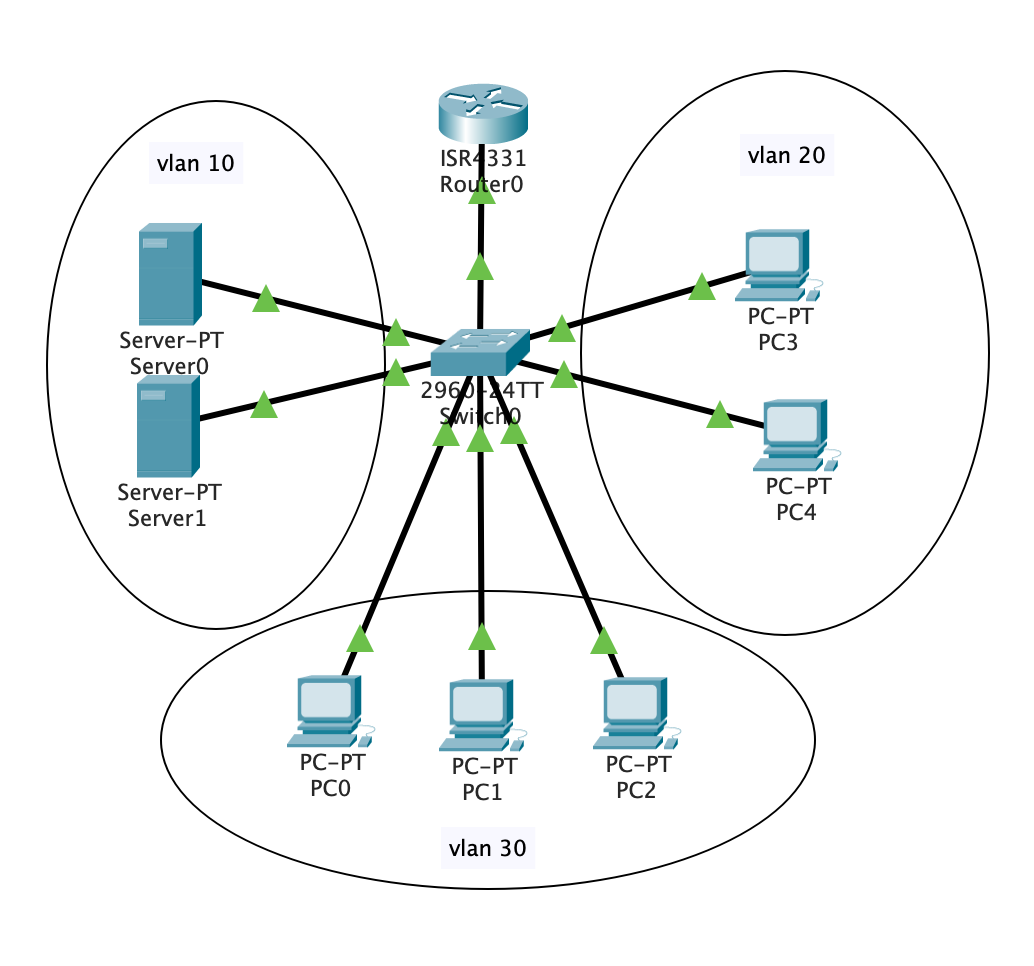
\includegraphics[width=0.7\linewidth]{inc/img/result.png}
\end{figure}

\end{document}
